% !TEX root = ../main.tex
% The area can only be sailed by metal ships, and they are dangerous af, filled with the illhveli (https://abookofcreatures.com/category/iceland/page/2/).

\begin{table*}[b]%
    \begin{DndTable}[width=\linewidth]{X}
        \centering
        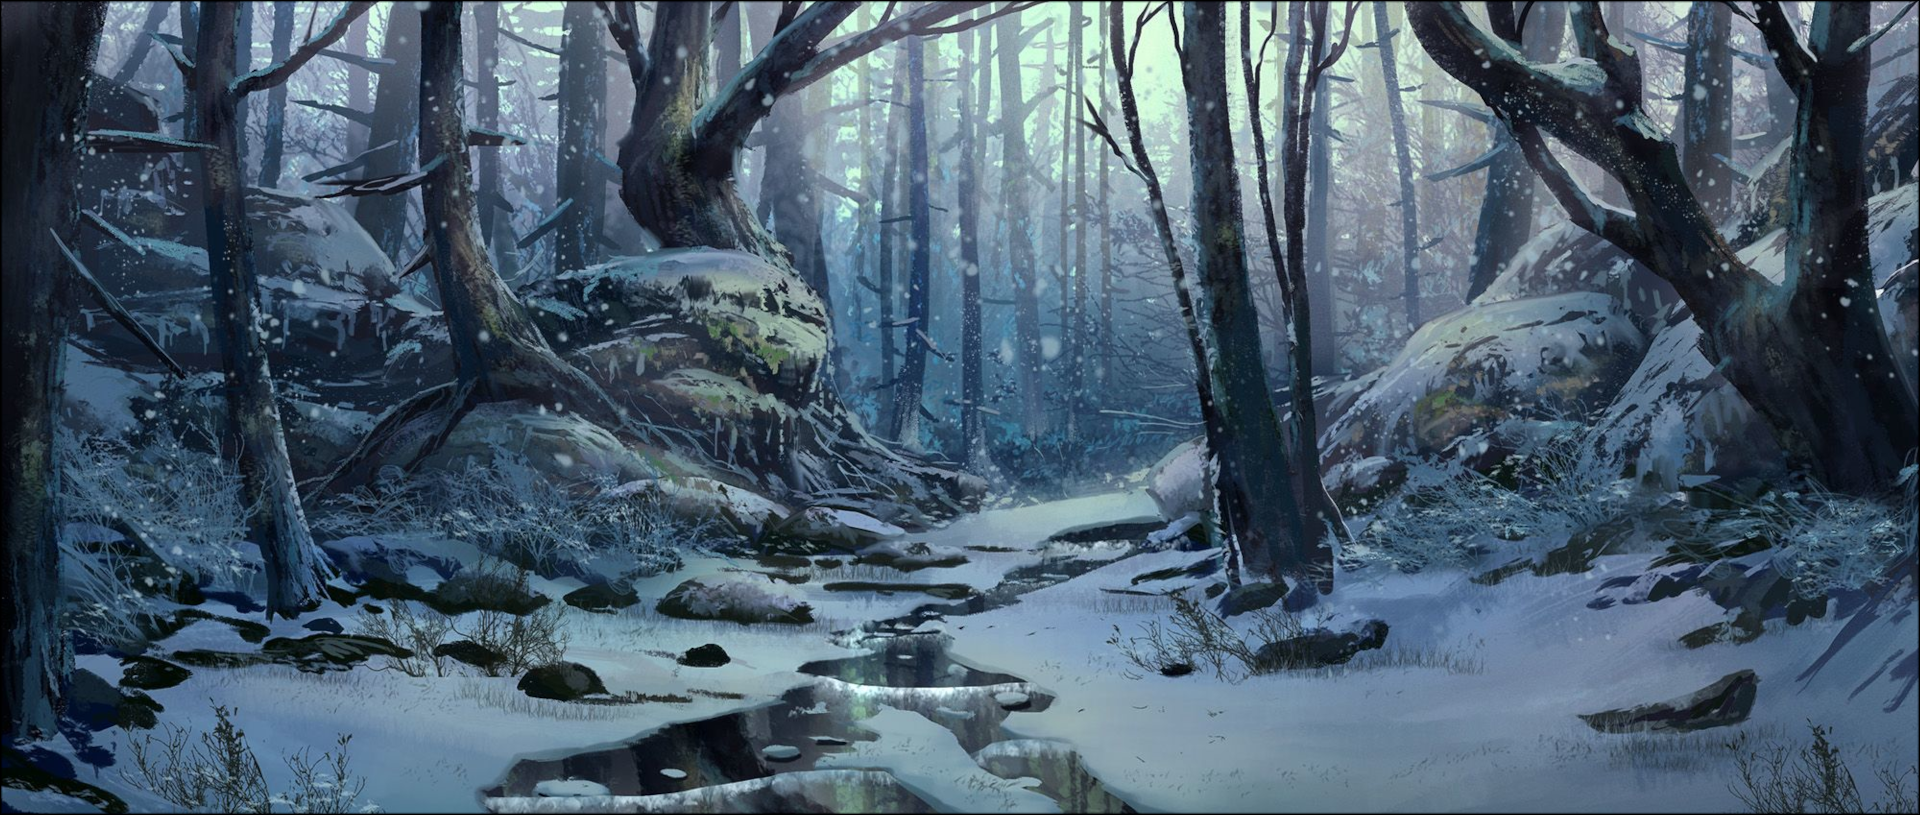
\includegraphics[width=0.95\textwidth]{01intro/img/11tallwoods.png} \
        \centering \large{\textbf{The Tallwoods}}
    \end{DndTable}
\end{table*}

\subsection*{Northern Territories}
The northmost region of Yuadrem, the Northern Territories are comprised by the Whitenorth, the Red Islands, the Tallwoods, the Blank Fields, and the Sulfur Lake.
The region is split by the Wall of Ice and Stone, a colossal mountain range that spans from coast to coast.

North of the wall is Whitenorth, an area split between the ancient ird kingdom of Krudzal and the territorial giants of Jatuunsa.
Its few inhabitants are beings of extreme resilience and fierceness, acclimated to the harsh habitat.
First among these are the giants, mountain-sized creature of stone, ever locked in war with Krudzal.

The middle of the region is characterized by the endless mists.
The area coincides with the north pole, and is inexplicably warm and misty despite its location.

To the west of Whitenorth is the Red Fjord, named so by its most common tree, the red maple.
The are is regarded sacred by the Krudzalians, who believe it to be the resting place of the sun god, Jua\~nanisz.
The fjord is currently occupied by Ribinhep, a uman nation ever standing up against the northerner irds.

Below the Wall of Ice and Stone are the Tallwoods and the Blank Fields.
The Tallwoods are an association of pine and redwood forest, using the mountains to hide from the cold winds.
The forests are devoid of civilized life, and the stone trolls who inhabit them make sure that they stay that way.

The Blank Fields are a vast, freezing tundra.
The low temperatures and strong winds in the area prohibit the growth of any vegetation.

The west of the fields are known as the Wurmlands, and they are solely inhabited by wurms.
Wurms are large reptile-like creatures that attack all foolish enough to approach their subterranean colonies.
The eastern portion of the land is filled to the brim with a variety of bughna gat tribes, ever in conflict for the large reserves of copper and coal in the mountains.

East to the fields is the Arctic Archipelago.
This cluster of islands separate the Whaler's Sea from the frigid ocean up north.
Mostly bare and desolate, the islets equally house ird, gat, uman, and zaloth settlements.

The strongest force in the archipelago is the Kaldrathal nation.
Having the only vessels strong enough to withstand the ship-sinking idzels, they regulate commerce in the entire archipelago.
% idzels or idzelal are inspired on Illhevi (https://abookofcreatures.com/category/iceland/page/2/).
